\section{管理属性}
\footnote{{\bf 重要:}如果你用过老版本的~Cytoscape就会发现属性的处理方式已经发生了
改编。其中,最重要的变化是属性不再是存放在当前目录或主目录的.cytoscape目录中,而是
保存在Cytoscape的会话文件中(后缀是.cys)。在.cytoscape目录下肯定会有一个
cytoscape.props文件,但这个文件只有当用户要求将但前属性保存为缺省属性时才会被修改。
除非实在是有什么特别的原因,否则还是用缺省设置比较好。}

用菜单上的Edit → Preferences → Properties…可以打开Cytoscape的属性编辑器,在这里可以
修改各种属性。对于一般的属性,都是保存在Cytoscape的会话文件中,所以只对当前会话有效。
只有将其设为缺省属性,或是用File → Export将其导出,才能在其他的会话中生效。

可以通过Add(添加)、Modify(修改)和Delete(删除)操作来配置Cytoscape的属性。
\begin{center}
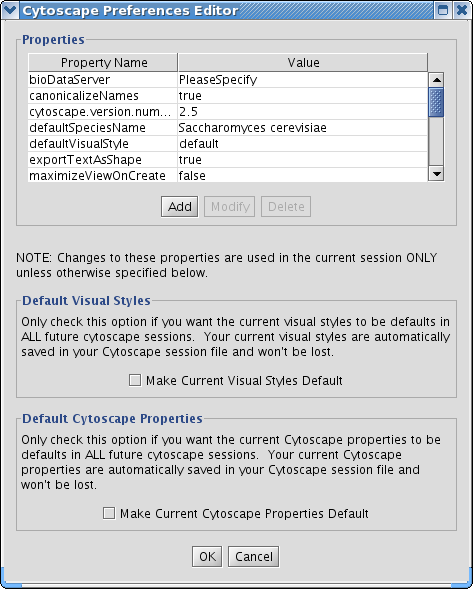
\includegraphics[width=\textwidth]{images/prefs_editor.png} 
 \end{center}